\chapter{The metric structure}\label{chap7:chap7}

\setcounter{section}{1}\label{chap7:chap7-sec1}


\setcounter{subsection}{0}


\subsection{}\label{chap7:7.1.1}\pageoriginale
In this chapter we assume that all the manifolds we consider are {\em
  connected.}


\noindent
{\bf 1. Identity of balls}

\subsection{}\label{chap7:7.1.2}

\begin{defi*}
For every pair of points $m$ and $n$ in $(M,g)$ we set
$$
\mathscr{P}(m,n)=\{C|C\text{ is a path from } m \text{ to } n\}.
$$
\end{defi*}

Since we have assumed that $M$ is connected it follows that $M$ is
arc wise connected and hence that
$$
\mathscr{P}(m,n)\neq \emptyset \; \forall m,n\in M.
$$
Now set
\begin{equation*}
d(m,n)=\inf_{C\in\mathscr{P}(m,n)}\lg(C).\tag{7.1.3}\label{chap7:7.1.3}
\end{equation*}

\setcounter{subsection}{3}
\subsection{}\label{chap7:7.1.4}

Then, since the length of a path is non-negative we have
$$
d(m,n)\geq 0;
$$
since every path from $m$ to $n$ gives rise to a path from $n$ to $m$
with the same length we have
$$
d(m,n)=d(n,m);
$$
and since a path from $m$ to $p$ and another from $p$ to $n$ give rise
to one from $m$ to $n$ we have
$$
d(m,n)\leq d(m,p)+d(p,n).
$$
Hence $d$ has all the properties of a metric structure except perhaps
the one which asserts that $d(m,n)=0$ only if $m=n$. Now we shall 
proceed \pageoriginale to show that this property is also valid; in
fact, we shall prove much more, namely, that locally geodesics realise
the distance $d$. 

\setcounter{subsection}{4}
\subsection{}\label{chap7:7.1.5}
Now throughout this article, let us fix a point $m$ and a positive
number $r$ such tht $\exp_{m}$ is $r$-O.K., and set:
$$
\lambda=(\exp_{m}|B(m,r))^{-1}.
$$

\setcounter{subsection}{5}

\subsection{}\label{chap7:7.1.6}

\begin{lemma*}
Let $n$ and $n'$ be points in $B(m,r)$ and let the map
$$
C:[0,t_{0}]\to M
$$
be a path such that
\begin{itemize}
\item[\rm i)] the image of $C$ does not contain $m$,

\item[\rm ii)] the image of $C$ lies wholly in $B(m,r)$.
\end{itemize}
Then we have
$$
\lg(C)\geq \,\big|\, ||\lambda(n')||-||\lambda(n)||\,\big|,
$$
and equality holds if and only if
\begin{itemize}
\item[\rm i)] the three points $0_{m}$, $\lambda(n)$ and $\lambda(n')$
  are in a straight line and

\item[\rm ii)] $\lambda\circ C$ lies in the segment
  $[\lambda(n),\lambda(n')]$ and is injective.
\end{itemize}
\end{lemma*}

\begin{proof}
Since $C$ is made up of finite number of curves and for any three real
numbers $a$, $b$ and $c$ we have
$$
|a-c|\leq |a-b|+|b-c|
$$
we need only prove that results for curves. So let us assume that $C$
is a curve:
$$
C\in D([0,t_{0}],M),
$$\pageoriginale
and set
\begin{equation*}
b=\lambda\circ C.\tag{7.1.8}\label{chap7:7.1.8}
\end{equation*}
Since by i) $0_{m}$ is not in the image of $C$ the map
$\dfrac{b}{||b||}$ makes sense and we write $x$ for it:
\begin{equation*}
x=\frac{b}{||b||}\tag{7.1.9}\label{chap7:7.1.9}
\end{equation*}
Then we have
\begin{equation*}
b'=||b||'\cdot \zeta^{-1}_{x}x+||b||x'.\tag{7.1.10}\label{chap7:7.1.10}
\end{equation*}
By the definition of $x$ we have $||x||=1$ and hence we have
$$
g(\zeta^{-1}_{x}x,x')=0
$$
and hence by Gauss' lemma (see (\ref{chap5:5.6.24})) we have
\begin{equation*}
g(\exp^{T}_{m}(||b||\cdot \zeta^{-1}_{x}x), \exp^{T}_{m}(||b||\cdot x'))=0.\tag{7.1.12}\label{chap7:7.1.12}
\end{equation*}
Now by (\ref{chap7:7.1.8}) and (\ref{chap7:7.1.10}) we have
\begin{align*}
&\qquad ||C'||^{2}=||\exp^{T}_{m}\circ b'||^{2}=\\
&  = ||\exp^{T}_{m}(||b||'\cdot\zeta^{-1}_{x}x)
  ||^{2}+2g(\exp^{T}_{m}(||b||'\zeta^{-1}_{x}x),\exp^{T}_{m}(||b||\cdot 
  x'))+ \tag{7.1.13}\label{chap7:7.1.13}\\
&\hspace{4cm} +||\exp^{T}(||b||\cdot x')||^{2}=\\
&= ||\exp^{T}_{m}(||b||'\cdot
  \zeta^{-1}_{x}x)||^{2}+||\exp^{T}_{m}(||b||x')||^{2},\quad\text{by
    \eqref{chap7:7.1.12}.} 
\end{align*}
But by (\ref{chap5:5.6.32}) i) we have
$$
||\exp^{T}_{m}(\zeta^{-1}_{x}x)||=||x||=1
$$
and hence
\begin{equation*}
||C'||^{2}=(||b||')^{2}+||\exp^{T}_{m}(||b||x')||^{2},\geq
(||b||')^{2}\tag{7.1.14}\label{chap7:7.1.14} 
\end{equation*}\pageoriginale
equality holding if and only if $||\exp^{T}_{m}x'||=0$.
\end{proof}

\setcounter{subsection}{14}
\subsection{}\label{chap7:7.1.15}
Since $\exp_{m}$ is $r$-O.K., this is equivalent to saying that
$$
||C'||\geq ||b||',
$$
and that equality holds if and only if $x'=0$.

Now we have
\begin{equation*}
\lg(C)=\int\limits^{t_{0}}_{0}||C'||\dt\geq
\int\limits^{t_{0}}_{0}||b||'\dt\geq \,\big|\, ||\lambda(n')||-||\lambda(n)||\,\big|.\tag{7.1.16}\label{chap7:7.1.16}
\end{equation*}

\setcounter{subsection}{16}
\subsection{}\label{chap7:7.1.17}
Further the last inequality becomes equality if and only if $||b||'$
is of the same sign.

\subsection{}\label{chap7:7.1.18}
Hence by (\ref{chap7:7.1.15}), \eqref{chap7:7.1.16} and (\ref{chap7:7.1.17}) we have
$$
\lg(C)\geq \,\big|\,||\lambda(n')||-||\lambda(n)||\,\big|
$$
where equality holds if and only if $x'=0$ and $||b||'$ is of the same
sign.

This means that equality holds if and only if $x$ is constant, and $b$
is injective. This means that $b$ should lie on the line joining
$0_{m}$ and $\lambda(n)$ and $b$ is injective.

\setcounter{subsection}{18}

\subsection{}\label{chap7:note7.1.19}

\begin{note*}
In the case $\lambda\circ C$ lies on a line through $0_{m}$ and is
injective we say, for simplicity, that $C$ is {\em a monotonic image
  by $\exp_{m}$ of the segment} $[(\lambda\circ C)(0),(\lambda\circ
  C)(t_{0})]$. 
\end{note*}

\setcounter{subsection}{19}

\subsection{}\label{chap7:7.1.20}

\begin{lemma*}
If\pageoriginale $0<r'<r$, then
$$
\exp(\overline{\ub{B}(m,r')})=\overline{B(m,r')}
$$
and the latter is a compact set.
\end{lemma*}

\begin{proof}
Since $\overline{\ub{B}(m,r')}$ is compact, $\exp$ continuous and $M$
Hausdorff, $\exp(\overline{\ub{B}(m,r')})$ is compact. In particular
$\exp(\overline{\ub{B}(m,r')})$ is closed.

But since $\exp(\ub{B}(m,r'))\subset \exp(\overline{\ub{B}(m,r')})$ it
follows that
$$
\overline{\exp(\ub{B}(m,r'))}\subset \exp(\overline{\ub{B}(m,r')}).
$$
In our case the other inclusion follows from the fact that $\exp$ is a
diffeomorphism on $\ub{B}(m,r)$.
\end{proof}


\subsection{}\label{chap7:7.1.21}

\begin{lemma*}
Let
\begin{figure}[H]
\centering
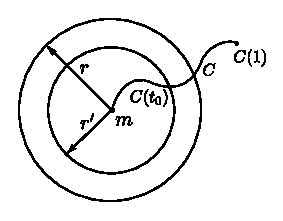
\includegraphics[scale=1.1]{figures/chap7-fig1.eps}
\end{figure}
$$
C:[0,1]\to M
$$
be a path in $M$ such that
$$
C(0)=m\quad\text{and}\quad C[(0,1])\not\subset B(m,r).
$$
Then $\forall r'\in ]0$, $r[$, \ $\exists\, t_{0}\in ]0$, $1[$ such
    that
$$
||\lambda(C(t_{0}))||=r'\quad\text{and}\quad C([0,t_{0}[)\subset B(m,r').
$$
\end{lemma*}

\begin{proof}
Let $J=\{s\in ]0$, $1[|C(s)\not\in B(m,r')\}$. By (\ref{chap7:7.1.20})
    and the continuity of $C$, $J$ is closed so that $t_{0}=\inf
    J>0$. We claim that $t_{0}$ has the property required above. By
    continuity:  $C(t_{0})=\lim_{t\xrightarrow[<]{}t_{0}}C(t)$; and
      $C(t)\subset B(m,r')\forall t<t_{0}$ since, $J$ being closed,
      $t_{0}\in J$.

Hence by (\ref{chap7:7.1.20}): $C(t_{0})\in
\overline{B(m,r')}=\exp(\overline{B(m,r')})$,
i.e. $||\lambda(C(t_{0}))||\leq r'$. But $t_{0}\in J$ implies that
$||\lambda(C(t_{0}))||\geq r'$. Further, \pageoriginale
$C([0,t_{0}[)\subset B(m,r')$ by definition of $t_{0}$.
\end{proof}

\subsection{}\label{chap7:7.1.22}

\begin{lemma*}
Let $n\in B(m,r)$ and let
$$
C:[0,t_{0}]\to M
$$
be a path, such that $C(0)=n$ and $C(t_{0})=m$ and whose image lies in
$B(m,r)$. Then
\begin{itemize}
\item[\rm i)] $\lg(C)\geq ||\lambda(n)||$ and

\item[\rm ii)] in {\rm i)} the equality holds if and only if $C$ is a
  monotonic image by $\exp_{m}$ of the segment $[\lambda(n),0_{m}]$. 
\end{itemize}
\end{lemma*}

\begin{proof}
Let $t_{1}=\inf_{t\in [0,t_{0}]}t|C(t)=m$.

Then for every sufficiently small positive number $\epsilon$ we have
\begin{equation*}
\lg(C)\geq
\lg(C|[0,t_{1}])\geq\lg(C|[0,t_{1}-\epsilon]).\tag{7.1.23}\label{chap7:7.1.23} 
\end{equation*}
Since $m\not\in C([0,t_{1}-\epsilon])$ by (\ref{chap7:7.1.6}) we have
\begin{equation*}
\lg(C|[0,t_{1}-\epsilon])\geq \,\big|\,||\lambda(n)||-||(\lambda\circ
C)(t_{1}-\epsilon)||\,\big|.\tag{7.1.24}\label{chap7:7.1.24} 
\end{equation*}
Since $\lg(C|[0,t])$ is a continuous function of $t$, taking limit as
$\epsilon\to 0$ we have
\begin{gather*}
\lg(C|[0,t_{1}])\geq \lim\,\big|\,||\lambda(n)||-||(\lambda\circ
C)(t_{1}-\epsilon)||\,\big|=\\
=\big|\,||\lambda(n)||-||\lambda(m)||\,\big|=||\lambda(n)||.\tag{7.1.25}\label{chap7:7.1.25} 
\end{gather*}
\end{proof}

\setcounter{subsection}{25}
\subsection{}\label{chap7:7.1.26}
To prove ii) let us note that if equality holds above then
\begin{itemize}
\item[(i)] $\lg(C|[t_{1},t_{0}])=0$ and hence $C([t_{1},t_{0}])=\{m\}$
  and

\item[(ii)] in the following sequence of inequalities equality should
  hold everywhere:
\begin{align*}
& \lg(C|[0,t_{1}])=\lg(C|[0, t_{1}-\epsilon])+\lg(C|[t_{1}-\epsilon,
  t_{1}])\\
& \geq \,\big|\,||\lambda(n)||-||(\lambda\circ
  C)(t_{1}-\epsilon)||\,\big|+||(\lambda\circ
  C)(t_{1}-\epsilon)||\text{ (by i) }\geq ||\lambda(n)||.
\end{align*}
Hence \pageoriginale it follows that the above inequalities are
equalities. Now from (\ref{chap7:7.1.6}) it follows from the first
equality that $\forall \epsilon$:
$$
(\lambda\circ C)(t_{1}-\epsilon)\in [0_{m},\lambda(n)]\quad\text{and
  that}\quad C|[0,t_{1}-\epsilon]
$$
is a monotone image by $\exp_{m}$ of the segment
$[\lambda(n),(\lambda\circ C)(t_{1}-\epsilon)]$.
\end{itemize}

\setcounter{subsection}{27}

\subsection{}\label{chap7:7.1.28}

\begin{lemma*}
Let $n$ be a point in $M$ and let
$$
C:[0,t_{0}]\to M
$$
be a path from $m$ to $n$ such that
$$
C([0,t_{0}])\not\subset B(m,r).
$$
Then
$$
\lg(C)\geq r.
$$
\end{lemma*}

\begin{proof}
Let $0<r'<r$. Then by (\ref{chap7:7.1.21}) $\exists\, t_{1}$ such that
$$
||\lambda(C(t_{1}))||=r'\quad\text{and}\quad C([0,t_{1}[)\subset B(m,r').
$$
Hence, by (\ref{chap7:7.1.22}) we have
$$
\lg(C)\geq \lg(C|[0,t_{1}])\geq ||\lambda(C(t_{1}))||=r'.
$$
This being true for every $r'<r$ we are through.
\end{proof}

\subsection{}\label{chap7:7.1.29}

\begin{theorem*}
Let $n\in B(m,r)$. Then
\begin{itemize}
\item[\rm i)] $d(m,n)=||\lambda(n)||$, and the geodesic
$$
\gamma_{\lambda(n)/||\lambda(n)||\,\big|\, [0,\lambda(n)]}
$$
realises the distance $d(m,n)$, and

\item[\rm ii)] it is the only one, i.e.\@ if $C\in\mathscr{P}(m,n)$ is
  such that $\lg(C)=d(m,n)$, then $C$ is a monotone image by
  $\exp_{m}$ of the segment $[0_{m},\lambda(n)]$.
\end{itemize}
\end{theorem*}

\begin{proof}
The \pageoriginale geodesic defined above has length $||\lambda(n)||$:
see \eqref{chap4:4.3.3}.\break Hence $d(m,n)\leq ||\lambda(n)||$.

But if $C\in\mathscr{P}(m,n)$ then by (\ref{chap7:7.1.22}) i) and
(\ref{chap7:7.1.28}) we have
$$
\lg(C)\geq ||\lambda(n)||.
$$
Hence $d(m,n)\geq ||\lambda(n)||$ and the first part follows.

To prove ii) let $C\in\mathscr{P}(m,n)$ and let
$\lg(C)=||\lambda(n)||$. Then by (\ref{chap7:7.1.28}) the image of $C$
lies in $B(m,r)$ and the part ii) states the same thing as
(\ref{chap7:7.1.22}) ii).
\end{proof}

\subsection{}\label{chap7:7.1.30}

\begin{notation*}
We set
$$
D(n,s)=\{n'\in M|d(n,n')<s\}.
$$
\end{notation*}

\subsection{}\label{chap7:7.1.31}

\begin{coro*}
If $\exp_{n}$ is $s$-O.K.\@ then
$$
B(n,s)=D(n,s).
$$
\end{coro*}

\begin{proof}
We have only to prove that $D(n,s)\subset B(n,s)$; so let $n'\in
D(n,s)$. Then $s'=d(n,n')<s$ and hence by the definition of $d$ there
exists a $C\in\mathscr{P}(n,n')$ such that $s'<\lg(C)<s$. Then by
(\ref{chap7:7.1.28}) the image of $C$ has to lie in $B(n,s)$. Hence
$$
n'\in B(n,s).
$$
\end{proof}

\section{The metric structure}\label{chap7:chap7-sec2}

\subsection{}\label{chap7:7.2.1}

\begin{prop*}
$d$ is a metric structure.
\end{prop*}

\begin{proof}
By (\ref{chap7:7.1.4}) we have only to prove that $d(m,n)=0$ implies
$m=n$. Now let $d(m,n)=0$. Then there exists an $r>0$ such that
$\exp_{m}$ is $r$-O.K. Hence by (\ref{chap7:7.1.31}) it follows that
$n\in B(m,r)$. Then by (\ref{chap7:7.1.29}) the result follows.
\end{proof}

\setcounter{subsection}{1}
\subsection{}\label{chap7:7.2.2}\pageoriginale

Whenever we consider the manifold $(M,g)$ as a metric space, {\em it
  is this metric we deal with}. Hence we speak of {\em distance}
without any mention of the metric structure involved. In particular,
we may speak of bounded sets, of completeness\ldots, in a r.m.\@
$(M,g)$. 

\subsection{}\label{chap7:rem7.2.3}

\begin{remark*}
Throughout we have assumed that $M$ is Hausdorff. This is a necessary
condition for a topology to come from a metric; Hausdorffness was used
only in proofs of (\ref{chap7:7.1.20}) and (\ref{chap7:7.1.21}).
\end{remark*}

\setcounter{subsection}{3}

\subsection{}\label{chap7:7.2.4}

\begin{prop*}
For a riemannian manifold $(M,g)$, the underlying topology of $M$
considered as a differentiable manifold and that induced by the metric
structure are the same.
\end{prop*}

\begin{proof}
Let $M$ be a point of $M$ and let $\exp_{m}$ be $r$-O.K. Then by
(\ref{chap7:7.1.31}) we have
$$
D(m,r')=B(m,r')\quad\text{if}\quad 0<r'<r.
$$
But every neighbourhood of $m$ in the topology induced by the metric
$d$ contains $D(m,r')$ for sufficiently small $r'$, and every
neighbourhood of $m$ in the original topology contains $B(m,r')$ for
sufficiently small $r'$ because $\lambda$ is a diffeomorphism. Hence
the neighbourhood system of $m$ in either topology is the same as that
in the other. Hence the result.
\end{proof}

The following is a direct consequence of the above proposition.

\setcounter{subsection}{4}

\subsection{}\label{chap7:7.2.5}

\begin{coro*}
The function $d:M\times M\to \mathbb{R}$ is continuous.
\end{coro*}

\subsection{}\label{chap7:7.2.6}

\begin{coro*}
We \pageoriginale have
$$
\overline{D(m,r)}=\{n\in M|d(m,n)\leq r\}\forall r>0.
$$
\end{coro*}

\begin{proof}
In view of (\ref{chap7:7.1.31}) and (\ref{chap7:7.2.5}) we have only to
prove that
$$
\{n\in M|d(m,n)=r\}\subset \overline{D(m,r)}.
$$
Suppose $n$ be such that $d(m,n)=r$; $\forall \epsilon>0$ (small
enough) $\exists\, C\in\mathscr{P}(m,n)$ such that $\lg(C)\leq
r+\epsilon$; by continuity we can find $n_{\epsilon}$ on the image of
$C$ with $d(m,n_{\epsilon})=r-\epsilon$ and so: $n_{\epsilon}\in
D(m,r)$; moreover:
$$
d(n,n_{\epsilon})\leq \lg(C|n\text{ to }
n_{\epsilon})=\lg(C)-\lg(C|m\text{ to } n_{\epsilon})\leq
r+\epsilon-d(m,n_{\epsilon})\leq 2\epsilon
$$
in particular $n_{\epsilon}\xrightarrow{\epsilon\to 0}n$, hence
$n\in\overline{D(m,r)}$. 
\end{proof}

\subsection{}\label{chap7:7.2.7}

\begin{example*}
Let $m$ be a point of $(\mathbb{S}^{d},\can)$ and $\sigma(m)$ its
antipodal point. Then since $\sigma(m)\not\in B(m,\pi)$ and $\exp_{m}$
is $\pi$-O.K.\@ (see (\ref{chap4:sec5})) we have\break $d(m,\sigma(m))\geq \pi$.
\end{example*}

But since there exists a great circular arc (geodesic) of length $\pi$
joining $m$ and $\sigma(m)$ we have
$$
d(m,\sigma(m))\leq \pi
$$
Hence
$$
d(m,\sigma(m))=\pi.
$$

\section{Nice balls}\label{chap7:chap7-sec3}

If $\exp_{m}$ is $r$-O.K.\@ then we know that $D(m,r)=B(m,r)$ and
further that for any point $n$ in $B(m,r)$ the distance $d(m,n)$ is
realised by a geodesic and that such a realisation is essentially
unique. Further\pageoriginale (see (\ref{chap2:2.6.8}) and (\ref{chap4:4.3.7})
we know that for sufficiently small $r$, $B(m,r)$ is convex and hence
any two points $n$ and $n'$ of it can be joined by a geodesic
$f_{n,n'}$ which is completely contained in $B(m,r)$ and that such a
curve is unique. So a natural question is whether $f_{n,n'}$ realises
the distance between $n$ and $n'$ and if so if it is the unique path
with that property. Before trying to answer this question we give a
name to the balls for which this (and more) is true.

\subsection{}\label{chap7:7.3.1}

\begin{defi*}
A ball $B(m,r)$ is called a {\em nice ball} if
\begin{itemize}
\item[\rm i)] $B(m,r)$ is convex

\item[\rm ii)] $\exp_{n}$ is $r$-O.K. $\forall n\in B(m,r)$ and

\item[\rm iii)] $\forall n$, $n'\in B(m,r)$ the geodesic $f_{n,n'}$
realises $d(n,n')$ uniquely, i.e., that $d(n,n')=\lg(f_{n,n'})$ and
upto a re parametrisation by a function $f_{n,n'}$ is the only path
that realises $d(n,n')$.
\end{itemize}
\end{defi*}

Now we shall prove that there are nice balls with assigned centres.

\subsection{}\label{chap7:7.3.2}

\begin{lemma*}
Suppose that $x\in U_{m}(M)$ and that $\exists\, t_{0}>0$ such that
\begin{itemize}
\item[\rm i)] $[0,t_{0}[\cdot x\subset \Omega$ and

\item[\rm ii)] there exists a sequence $\{t_{n}\}$ of numbers in
  $[0,t_{0}[$ and a point $p$ in $M$ such that $t_{n}\to t_{0}$ and
    $\gamma_{x}(t_{n})\to p$ as $n-\infty$.
\end{itemize}
Then $t_{0}x\in \Omega$.
\end{lemma*}

\begin{proof}
\begin{itemize}
\item[a)] First \pageoriginale let us prove that
$$
\gamma_{x}(t)\to P\quad\text{as}\quad t\to t_{0}.
$$
Since $d$ is a metric it is enough to prove that
$d(\gamma_{x}(t),p)\xrightarrow{t\to t_{0}} 0$.

We have
$$
d(\gamma_{x}(t),p)\leq
d(\gamma_{x}(t),\gamma_{x}(t_{n}))+d(\gamma_{x}(t_{n}),p). 
$$
Since $d$ is continuous by (\ref{chap7:7.2.5}) and since
$\gamma_{x}(t_{n})$ tends to $p$ as $n$ tends to infinity by
hypothesis the second term on the right hand side tends to zero as $n$
tends to infinity. Further, by \eqref{chap4:4.3.3}, 
$$
\lg(\gamma_{x}|[t_{n},t])\leq |t-t_{n}|
$$
since $x\in U_{m}(N)$. Hence
$$
\lg(\gamma_{x}|[t_{n},t])\leq |t-t_{0}|+|t_{0}-t_{n}|,
$$
and hence
$$
d(\gamma_{x}(t),p)\leq d(\gamma_{x}(t_{n}),p)+|t_{n}-t_{0}|+|t-t_{0}|.
$$
So for $t$ in $[t_{0}-\epsilon,t_{0}]$ we have
$$
d(\gamma_{x}(t),p)\leq d(\gamma_{x}(t_{n}),p)+|t_{n}-t_{0}|+\epsilon,
$$
and hence the result.

\item[b)] Let $W$ be a convex ball with centre at $p$, and let
$$
s:W\times W\to {}^{W}\Omega
$$
\begin{figure}[H]
\centering
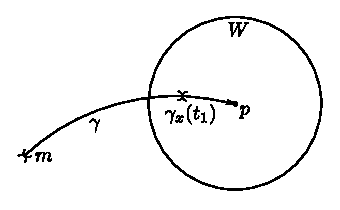
\includegraphics{figures/chap7-fig2.eps}
\end{figure}
\end{itemize}
be the associated map (see (\ref{chap2:sec6})). Since
$\gamma_{x}(t)\xrightarrow{t\to t_{0}} t_{0}$ then \pageoriginale
$\exists\, t_{1}\in[0,t_{0}[$ such that
$$
\gamma_{x}([t_{1},t_{0})\subset W.
$$
Set $u=\gamma'_{x}(t_{1})$; by (\ref{chap2:2.6.6}) we have
$$
s(\gamma_{x}(t_{1}), \gamma_{x}(t))=(t-t_{1})\cdot
u\quad\text{for}\quad t_{1}<t<t_{0}. 
$$
Now $s$ being continuous we have
$$
s(\gamma_{x}(t_{1}),p)=\lim\limits_{t\to
  t_{0}}s(\gamma_{x}(t_{1}),\gamma_{x}(t))=\lim\limits_{t\to
  t_{0}}(t-t_{1})\cdot u=(t_{0}-t_{1})\cdot u.
$$
Hence by the definition of $s$ it follows that $(t_{0}-t_{1})\cdot
u\in {}^{W}\Omega$. Since ${}^{W}\Omega$ is an open set there exists a
positive number $\delta$ such that
$$
[t_{1},t_{0}+\delta]\cdot u\subset{}^{W}\Omega
$$
and since ${}^{W}\Omega\subset\Omega$ we have
$$
[t_{1},t_{0}+\delta]\cdot u\subset\Omega.
$$
But this means simply that the geodesics $\gamma_{x}$ can be extended
to the point $\exp(t_{0}+\delta)\cdot x$ and hence $t_{0}\cdot x\in\Omega$.
\end{proof}

\begin{lemma*}[7.3.2 bis]\label{chap7:7.3.2bis}
Let $m$ be a point of $(M,g)$ such that $\exp_{m}$ is $r$-O.K. Then
$$
\Omega\supset \ub{B}(n,r-d(m,n))\cdot nB(m,r).
$$
\end{lemma*}

\begin{proof}
Let $n\in B(m,r)$, $x\in U_{n}(M)$.
\begin{figure}[H]
\centering
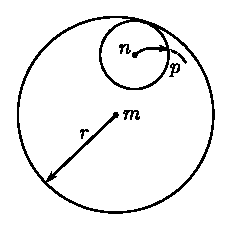
\includegraphics{figures/chap7-fig3.eps}
\end{figure}
\noindent
We have to show that (see (\ref{chap0:0.6.4}))
$$
s=t^{+}_{G}(x)\geq r-d(m,n).
$$
We suppose the contrary and deduce a contradiction.

Let\pageoriginale
$$
s<r-d(m,n).
$$
Then setting $r'=d(m,n)+s$ we have $r'<r$.

Further $\forall t\in [0,s]$, we have
\begin{align*}
d(m,\exp(tx)) &\leq d(m,n)+d(n,\exp(tx))\\
              &\leq d(m,n)+s=r'<r.
\end{align*}
Now we take a sequence $\{t_{n}\}$ of numbers in $[0,s[$ tending to
    $s$ as $n\to \infty$. Then the sequence of points $\{\exp
    t_{n}x\}$ lies in $B(m,r')$ and since $\overline{\ub{B}(m,r')}$ is
    compact (see (\ref{chap7:7.1.20})) and
    $\overline{\ub{B}(m,r')}=\exp(\overline{\ub{B}(m,r')})$, a
    sub sequence of $\{\exp t_{n}x\}$ converges to a point $p\in
    B(m,r)$. Hence the above lemma gives that
$$
s\cdot x\in\Omega
$$
and this contradicts the definition of $s=t^{+}_{G}(x)$.
\end{proof}

\setcounter{subsection}{2}

\subsection{}\label{chap7:7.3.3}

\begin{theorem*}
For every $m$ of $M$ there exists an $r>0$ such that $B(m,r)$ is a
nice ball.
\end{theorem*}

\begin{proof}
Let $r_{1}$ be a positive number such that $\exp_{m}$ is
$r_{1}$-O.K\@. and\break $B(m,r_{1})$ is convex.

We claim that we have only to set $r=\dfrac{r_{1}}{3}$.
\begin{itemize}
\item[\rm i)] By (\ref{chap4:4.3.7}) $B(m,r)$ is convex.

\item[\rm ii)] Let $n$ be in $B(m,r)$. Then, by (\ref{chap7:7.1.31}) we
  get $d(m,n)<r$. Hence by (\ref{chap7:7.3.2bis}):
$$
\ub{B}\left(n,r_{1}-\frac{r_{1}}{3}\right)=\ub{B}(n,2r)\subset \Omega.
$$
Further by (\ref{chap2:2.6.5}) $\exp_{n}$ is $2r$-O.K.\@ and in
particular $r$-O.K.

\item[\rm iii)] Let $n$, $n'\in B(m,r)$. Then $d(n,n')\leq
  d(n,m)+d(m,n')<2r$ so we are through because of (\ref{chap7:7.1.29}).
\end{itemize}
\end{proof}

\subsection{}\label{chap7:7.3.4}

\begin{coro*}
Let \pageoriginale $K$ be a compact subset of $M$. Then there exists
$\delta>0$ such that $\exp_{m}$ is $\delta-\text{O.K.}\forall m\in K$.
\end{coro*}

\begin{proof}
By the compactness of $K$ we can cover it with a finite number of nice
balls $B(m_{i},r_{i})$. Then we are through if we set
$\delta=\inf_{i}r_{i}$. 
\end{proof}

\subsection{}\label{chap7:7.3.5}

\begin{coro*}
Let $n$, $n'\in M$ and $C\in\mathscr{P}(n,n')$ be such that
$$
\lg(C)=d(n,n').
$$
Then (upto injective re parametrisation) $C$ is a geodesic.
\end{coro*}

\begin{proof}
Let $C=\{[a_{i},b_{i}]\subset I_{i},f_{i}\in D(I_{i},M)\}$.

Since being a geodesic is a local property, it is enough to show that
for each point $n=f_{i}(t_{i})$ there is a neighbourhood of $t_{i}$ in
which $C$ is a geodesic. Now let $B(n,r')$ be a nice ball.
\begin{figure}[H]
\centering
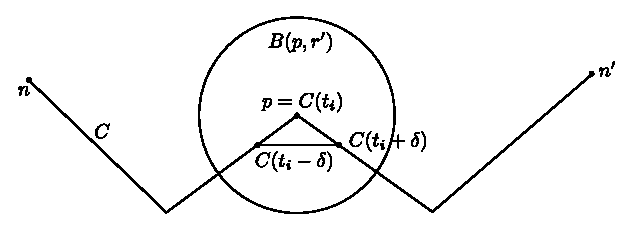
\includegraphics{figures/chap7-fig4.eps}
\end{figure}
\noindent
Then since $C$ is continuous there exists a $\delta>0$ such that
$$
C([t_{i}-\delta,t_{i}+\delta])\subset B(n,r').
$$
Now let $f$ be the geodesic in $B(n,r')$ from $C(t_{i}-\delta)$ to
$C(t_{i}+\delta)$. 

Then by the definition of a nice ball, if $C$ restricted to
$(t_{i}-\delta, t_{i}+\delta)$ were not a geodesic, we would have
$\lg(C)>\lg(f)$, and hence replacing that part of $C$ by $f$ we would
get
$$
d(n,n')<\lg(C|[a_{1},t_{i}-\delta])+\lg(C|[t_{i}+\delta,b_{k}])+\lg
f<\lg(C),
$$
a contradiction. 
\end{proof}

As \pageoriginale an application of the above corollary we prove the
following result called {\em ``the corner condition''} or {\em ``the
  strict triangle inequality''.}

\setcounter{subsection}{5}
\subsection{}\label{chap7:7.3.6}


\begin{application*}
Let $f$ be a geodesic from $n$ to $n'$ and $g$ be a geodesic from $n'$
to $n''$ both being parametrised by the arc length. Then if
$f'(n')\neq g'(n')$ then $d(n,n'')<d(n,n')+d(n',n'')$. 
\end{application*}

\begin{proof}
For if $d(n,n'')=d(n,n')+d(n',n'')$ the above corollary gives that the
path from $n$ to $n''$ given by $f$ from $n$ to $n'$ together with $g$
from $n'$ to $n''$ is a geodesic. Then since both are parametrised by
arc length we should have $f'(n')=g'(n')$.
\end{proof}

\setcounter{subsection}{6}
\subsection{}\label{chap7:7.3.7}
We insert here a result we will need later on (see (\ref{chap8:sec10})). Let
$B(m,r)$ be a nice ball, $n$, $n'\in B(m,r)$. We associate to $n$,
$n'$ and $t\in [0,1]$ the point $(n,n',t)$ defined as follows:
$(n,n',t)$ is on {\em the} geodesic from $n$ to $n'$ in $B(m,r)$ and
such that $d(n,(n,n',t))=t\cdot d(n,n')$. In particular
$(n,n',\frac{1}{2})$ can be called the {\em mid-point} of $n$, $n'$.


\subsection{}\label{chap7:7.3.8}

\begin{prop*}
Let $(M,g)$ be an r.m.\@ such that $A(M)\subset ]-\infty,0]$ and let
$B(m,r)$ be a nice ball. Then
$$
d((m,n,t),(m,n',t))\leq t\cdot d(n,n')\;\forall t\in [0,1],\forall
n,n'\in B(m,r).
$$
\end{prop*}

\begin{proof}
Set $1=d(n,n')$ and define a one parameter family of curves
$f:[0,1]\times [0,1]\to M$ by: 
$$
f(t,\alpha)=\left(m,\left(n,n',\frac{\alpha}{1}\right),t\right).
$$
\begin{figure}[H]
\centering
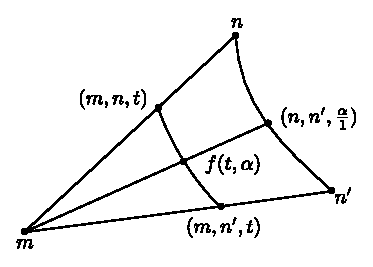
\includegraphics{figures/chap7-fig5.eps}
\end{figure}
\noindent
Then with the notations of (\ref{chap2:sec8}): each $f_{\alpha}$ is a
geodesic, so $t\to \uub{Q}(t,\alpha)$ is a Jacobi field along
$f_{\alpha}$. By \pageoriginale $A(M)\subset ]-\infty$, $0]$ and
  (\ref{chap5:5.6.19}) we have $\frac{1}{2}\dfrac{d^{2}}{\dt^{2}}(E\circ
  \uub{Q})\geq E\circ D_{P}\uub{Q}$. We normalize $\uub{Q}$ in $H$, so
  that $\uub{Q}=\varphi\cdot H$ with $E\circ H=1$. Then:
  $g(H,D_{P}H)=0$ so that $E\circ
  D_{P}\uub{Q}=\left(\dfrac{d\varphi}{\dt}\right)^{2}+E\circ D_{P}H\geq
  \left(\dfrac{d\varphi}{\dt}\right)^{2}$ as
  $E\circ\uub{Q}=\varphi^{2}$, we get
  $\dfrac{d^{2}\varphi}{\dt^{2}}>0$. So $\varphi$ is a positive
  function, vanishing at $t=0$, in a particular $\varphi(t)\leq
  t\cdot\varphi(1)$, which reads $||\uub{Q}(t,\alpha)||\leq
  t||\uub{Q}(1,\alpha)||$. But $\uub{Q}(t,\alpha)$ is the speed of the
  transverse curve $c_{t}$ which connects $(m,n,t)$ and $(m,n',t)$ so:
  $d((m,n,t),(m,n',t))\leq
  \lg(c_{t})=\int^{1}_{0}||\uub{Q}(t,\alpha)||d\alpha$
$$
\leq
\int\limits^{1}_{0}t||\uub{Q}(1,\alpha)||d\alpha=t\cdot\lg(c_{1})=t\cdot
d(n,n'). 
$$
\end{proof}

\section{Hopf-Rinow theorem}\label{chap7:chap7-sec4}

\subsection{}\label{chap7:defi7.4.1}

\begin{defi*}
We set:
$\mathscr{T}(n,n')=\{C\in\mathscr{P}(n,n')|\lg(C)=d(n,n')\}$. Then
each path is a geodesic by (\ref{chap7:7.3.5}) and we will always
normalize it requiring it to be parametrized by its arc length. We put
only such paths in $\mathscr{T}(n,n')$. 
\end{defi*}

Let us note that, in general, $\mathscr{T}(n,n')$ is neither empty nor
consists of a single element, as can be seen from the manifold
($\mathbb{S}^{d}-p$, can) obtained from the sphere $\mathbb{S}^d$ by
deleting one point $p$: $\mathscr{T}(m,m')=\emptyset$ and
$\mathscr{T}(n,n')$ has continuous elements.
\begin{figure}[H]
\centering
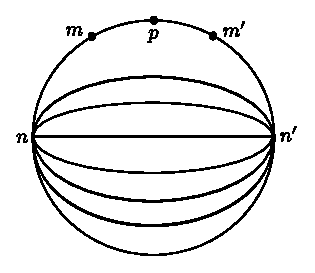
\includegraphics{figures/chap7-fig6.eps}
\end{figure}

\setcounter{subsection}{1}
\subsection{}\label{chap7:7.4.2}\pageoriginale

Suppose that $\mathscr{T}(n,n')$ is non-empty. Then there exists an
$$
f:[0,1]\to M
$$
such that $f$ is a geodesic parametrised by the arc length, $f(0)=n$
and $f(1)=n'$. Let $x$ be the initial speed of $f$. Then the curve
$$
t\to \gamma_{x}(t)=\exp(tx)
$$
is a geodesic through $n$ with the initial speed $x$. Hence it follows
that $f$ is the restriction of $\gamma_{x}$ to $[0,1]$ and hence that
\begin{gather*}
n'=\exp(1\;x)\\
\text{i.e.}\qquad
n'\in\exp(\overline{\ub{B}(n,1)})\quad\text{and}\quad 1\cdot x\in\Omega,
\end{gather*}
since $f$ is parametrised by the arc length and hence $x$ is a unit
vector.

\subsection{}\label{chap7:7.4.3}

\begin{theorem}[Hopf-Rinow]
The following four properties are equivalent.
\begin{itemize}
\item[\rm i)] Every closed bounded set in $M$ is compact.

\item[\rm ii)] $M$ is complete.

\item[\rm iii)] $\Omega=T(M)$.

\item[\rm iv)] There exists a point $m$ in $M$ such that
  $T_{m}(M)\subset \Omega$.
\end{itemize}
\end{theorem}

\begin{proof}
We shall prove that
$$
{\rm (i) }\Rightarrow {\rm (ii) } \Rightarrow {\rm (iii) } \Rightarrow
{\rm (iv) }\Rightarrow {\rm (i)}.
$$
Since every Cauchy sequence is bounded the first implication is clear.
\end{proof}

To prove that $\Omega=T(M)$ it is enough to show that $\forall x\in
U(M)$ one has $t^{+}(x)=+\infty$.

Suppose $t^{+}(x)<\infty$; then there exists a Cauchy sequence
$$
\{t_{n}\}\subset [0,t^{+}(x)[
$$
such that\pageoriginale
\begin{gather*}
t_{n}\to t^{+}(x).\\
n\to \infty
\end{gather*}
Then we have: $d(\exp(t_{i}\cdot x),\exp(t_{j}\cdot x))\leq
|t_{i}-t_{j}|\cdot ||x||=|t_{i}-t_{j}|$ and hence $\exp t_{i}x$ is a
Cauchy sequence. So if $M$ is complete this sequence has a limit point
and an application of (\ref{chap7:7.3.2}) gives the second implication
\begin{quote}
The third implication is clear.

So we are left with proving the fourth implication. It will
\end{quote}
be a consequence of the following:

\subsection{}\label{chap7:prop7.4.4}

\begin{prop*}
If for some point $m$ in $M$
$$
T_{m}(M)\subset \Omega
$$
then
$$
\mathscr{T}(m,n)\neq \emptyset\quad\forall n\in M
$$
(In fact if $K$ is closed and bounded, $\exists\, r|K\subset
\overline{D(m,r)}$ but $\overline{D(m,r)}\subset
\exp(\overline{\ub{B}(m,r)})$ which is compact. So $K$ is closed in a
compact, hence compact)
\end{prop*}

\noindent
{\bf Proof of the proposition.} Set:
$$
D_{t}=\overline{D(m,t)}, F_{t}=\{n\in D_{t}|\mathscr{T}(m,n)\neq
\emptyset\}, I=\{t\geq 0|D_{t}=F_{t}\}.
$$
We remark that $F_{t}$ is closed: this follows easily from the fact
that $\Omega\supset T_{m}(M)$. Moreover $\exists\, r|I\supset [0,r]$,
for (\ref{chap7:7.1.29}) implies that $I\supset [0,r]$ as soon as
$\exp_{m}$ is $r$-O.K. We are going to prove that $I$ is both closed
and open.

\subsection{}\label{chap7:7.4.5}


\begin{lemma*}
Let \pageoriginale $r\in I$, $n\not\in D_{r}$; then $\exists\, p\in
D_{r}$ such that $d(m,p)=r$ and $d(m,n)=d(m,p)+d(p,n)$. 
\end{lemma*}

\noindent
{\bf Proof of the lemma.}~$D_{r}=F_{r}$ being compact, $\exists\, p\in
D_{r}$ such that
$$
d(p,n)=\inf\{d(n,q)|q\in D_{r}\}.
$$
{\em We claim}:~$p$ is the right one. For $\forall \epsilon>0$,
$\exists\, C\in\mathscr{P}(m,n)$ such that
$\lg(C)<d(m,n)+\epsilon$. Because $t\to d(m,C(t))$ is continuous
$\exists\, b$ such that $d(C(b),m)=r$.
\begin{figure}[H]
\centering
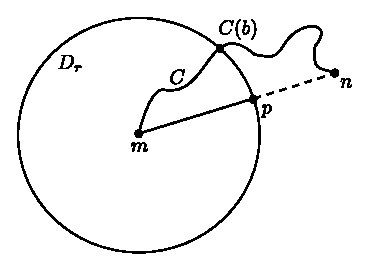
\includegraphics{figures/chap7-fig7.eps}
\end{figure}

But:
\begin{align*}
& r+d(p,n)\leq r+d(C(b),n)\leq\\
&\leq\lg(C|m\text{ \  to \ }C(b))+\lg(C|C(b)\text{ \ to
    \ }n)=\lg(C)\leq\\
&\leq \epsilon+d(m,n)\\
\text{so} &: r+d(p,n)\leq \epsilon+d(m,n). 
\end{align*}

Letting $\epsilon\to 0$, we obtain
$$
r+d(p,n)\leq d(m,n)\leq d(m,p)+d(p,n)\leq r+d(p,n)
$$
hence
$$
d(m,p)+d(p,n)=d(m,n).
$$

\setcounter{subsection}{5}
\subsection{}\label{chap7:7.4.6}
$I$ is closed. Let $\{r_{i}\}\subset I$ be such that
$\lim\limits_{i\to \infty} r_{i}=r$, and \pageoriginale let $n\in
D_{r}$. If $d(m,n)<r$, then $\exists\, i|d(m,n)<r_{i}$ so
$\mathscr{T}(m,n)\neq \emptyset$. If $d(m,n)=r$ and if $n\not\in
D_{r_{i}}\forall i$ then by (\ref{chap7:7.4.5}) $\exists\, p_{i}\in
D_{r_{i}}$ with $d(m,n)=r=r_{i}+d(p_{i},n)$. When $i\to
\infty:d(p_{i},n)\to 0$, so $p_{i}\to n$. But $\forall i:p_{i}\in
F_{r_{i}}\subset F_{r}$ and $F_{r}$ is closed; so $n\in F_{r}$. In any
case then $n\in F_{r}$ i.e.\@ $D_{r}=F_{r}$.

\subsection{}\label{chap7:7.4.7}
{\em $I$ is open.} Suppose $I=[0,r_{0}]$ and get a contradiction as
follows. From the compactness of $F_{r_{0}}=D_{r_{0}}$ we can by
(\ref{chap7:7.3.4}) find $r>0$ such that $\exp_{p}$ is $r$-O.K. $\forall
p\in D_{r_{0}}$.

\noindent
{\bf Claim:}~$F_{r'}=D_{r'}\forall r'|r_{0}<r'<r_{0}+r$. In fact if
$n\in M$ with $r_{0}<d(m,n)<r'<r_{0}+r$ then $n\not\in D_{r_{0}}$. By
(\ref{chap7:7.4.5}) $\exists\, p$ with $d(m,p)=r_{0}$ and
$d(m,p)+d(p,n)=d(m,n)$ hence $d(p,n)<r_{0}+r-r=r$ so by
(\ref{chap7:7.1.29}) $\exists\, g\in\mathscr{T}(p,n)$ and $\exists\,
f\in\mathscr{T}(m,n)$ and $\lg(f\cup g)=d(m,n)$ so $f\cup
g\in\mathscr{T}(m,n)$. Let us note the results proved in the course of
the proof of the Hopf-Rinow theorem as corollaries.

\subsection{}\label{chap7:7.4.8}

\begin{coro*}
If $(M,g)$ satisfies any one of the four equivalent conditions of
(\ref{chap7:7.4.3}) then
$$
\mathscr{T}(n,n')\neq \cdot \emptyset\quad\forall\quad n,n'\in M.
$$
\end{coro*}


\subsection{}\label{chap7:7.4.9}

\begin{coro*}
If $(M,g)$ satisfies any one of the four equivalent conditions of
\eqref{chap6:6.4.3} then for any point $n$ of $M$ and every $s>0$ we have
$$
D(n,s)=\exp(\ub{B},(n,s)).
$$
\end{coro*}

\begin{coro*}\label{chap7:7.4.10}
If $(M,g)$ is complete and $n$, $n'$ and $n''$ are points of $M$ such
that $d(n,n'')=d(n,n')+d(n',n'')$ then $\exists\, f\in
\mathscr{T}(n,n')$ such that the image set of $f$ contains $n'$.
\end{coro*}

For \pageoriginale one can take $f_{1}\in\mathscr{T}(n,n')$ and
$f_{2}\in \mathscr{T}(n',n'')$ and joining them get the element
$f_{1}\cup f_{2}$ of $\mathscr{T}(n,n'')$ by (\ref{chap7:7.3.5}). 

\subsection{}\label{chap7:7.4.11}

\begin{remarks*}
\begin{itemize}
\item[1)] The converse of (\ref{chap7:7.4.8}) is false. For example in a
  euclidean ball for any two points $n$ and $n'$ we have
  $\mathscr{T}(n,n')\neq \emptyset$. But it is not complete.

\item[2)] The completeness, in general, depends on $g$. For example
  the manifold $\mathbb{S}^{1}\times \mathbb{R}$ with the product
  r.s.\@ is homeomorphic to the manifold $\mathbb{R}^{2}-\{0\}$ with
  the r.s.\@ induced from $\mathbb{R}^{2}$. But the former is complete
  and the later is not. But if $M$ is compact then for any r.s.\@
  $g(M,g)$ is complete by (\ref{chap7:7.2.4}) and hence complete.

\item[3)] The Hopf-Rinow theorem and corollary (\ref{chap7:7.4.7}) are the
  starting\break points for obtaining global results in riemannian
  geometry. We shall give typical examples in the next articles and in
  Chapter VIII.
\end{itemize}
\end{remarks*}

\setcounter{subsection}{11}
\subsection{}\label{chap7:7.4.12}
Symmetric pairs give r.m.'s. $M=G/K$ which are always complete: in
fact use (\ref{chap4:4.4.1}) to check (iv) in (\ref{chap7:7.4.3}) for
$m=m_{0}=p(e)$. 

\section{A covering criterion}\label{chap7:chap7-sec5}

\subsection{}\label{chap7:7.5.1}

\begin{prop*}
Let two r.m.'s $(M,g)$ and $(N,h)$ of the same dimension and a map
$p\in D(M,N)$ be such that
\begin{itemize}
\item[\rm i)] $p$ is onto,

\item[\rm ii)] $g=p^{\ast}h$,

\item[\rm iii)] $(M,g)$ is complete.
\end{itemize}
Then $p$ is a covering map.
\end{prop*}

\begin{proof}
By the definition of a covering map we have to show that given any
point $n$ of $N$ there exists a neighbourhood $V$ of $n$ such that
each connected component of $p^{-1}(V)$ is homeomorphic to $V$ through
$p$. We \pageoriginale shall show that if $\exp_{n}$ is $s$-O.K., then
$B(n,s)$ is a neighbourhood with the above property.
\begin{itemize}
\item[a)] Let $m\in p^{-1}(n)$; then from ii) it follows that
$p^{T}_{m}$ is injective, and since the manifolds are of the same
dimension that $p^{T}_{m}$ is bijective. Hence by (ii) it follows that
$p^{T}_{m}$ is a euclidean isomorphism between $T_{m}(M)$ and
$T_{n}(N)$. Let us set
$$
\lambda=(\exp_{n}|B(n,s))^{-1}.
$$
Then since $(M,g)$ is complete and hence $T(M)={}^{M}\Omega$ we can
define the map
$$
q={}^{M}\exp\circ (p^{T}_{m})^{-1}\circ \lambda:B(n,s)\to M.
$$
Let us note, since $p^{T}_{m}$ is a euclidean isomorphism, that the
image of $q$ is $B(m,s)$. Further since $g=p^{\ast}h$ by
(\ref{chap4:4.2.6}) we have
$$
p\circ {}^{M}\exp ={}^{N}\exp \circ p^{T}_{m}
$$
and hence
\begin{align*}
(p^{T}_{m})^{-1}\circ\lambda\circ p\circ
{}^{M}\exp&=(p^{T}_{m})^{-1}\circ\lambda\circ {}^{N}\exp\circ
p^{T}_{m}\\
&=(p^{T}_{m})^{-1}\circ \id_{\ub{B}(n,s)}\circ p^{T}_{m}=\id_{\ub{B}(m,s)}
\end{align*}
and hence $(p^{T}_{m})^{-1}\circ \lambda\circ p$ is the inverse of
${}^{M}\exp$ on $\ub{B}(m,s)$. In particular ${}^{M}\exp$ is $s$-O.K.,
and $p$ and $q$ are diffeomorphisms which are inverses of each other.

\item[b)] Now suppose that $m'$ is any point in $p^{-1}(n)$. Let $u\in
  B(m,s)\cap B(m',s)$. Since by a) $\exp_{m}$ is $s$-O.K, by
  (\ref{chap7:7.1.29}) there is a unique geodesic $\gamma_{1}$
  parametrised by the arc length from $m$ to $u$ realising the
  distance between $m$ and $u$, and a similar one $\gamma_{2}$
  from \pageoriginale $m'$ to $u$. Then since $p$ is a local isometry
  by ii)~it follows that $p\circ\gamma_{1}$ is a geodesic
  (parametrised by the arc length) realising the distance between $n$
  and $p(u)$, and $p\circ\gamma_{2}$ is also one such. Hence
  $p\circ\gamma_{1}=p\circ\gamma_{2}$. Therefore $\gamma_{1}$ and
  $\gamma_{2}$ are lifts of the same curve having a common point
  $u$. Since $p$ is local diffeomorphism $\gamma_{1}=\gamma_{2}$ and
  hence $m=\gamma_{1}(0)=\gamma_{2}(0)=m'$. So we have $B(m,s)\cap
  B(m,s')=\emptyset$ as soon as $m\neq m'$.

\item[\rm c)] We now prove that
$$
p^{-1}(B(n,s))=\bigcup_{m\in p^{-1}(n)}B(m,s).
$$
\begin{figure}[H]
\centering
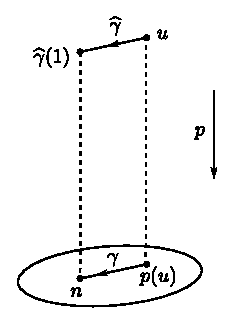
\includegraphics{figures/chap7-fig8.eps}
\end{figure}

Let $u\in p^{-1}(B(n,s))$ and let
$$
\gamma:[0,1]\to N
$$
be an element of $\mathscr{T}(p(U),n)$ and $\widehat{\gamma}$ be the
geodesic in $(M,g)$ such that
$$
\widehat{\gamma}'(0)=(p^{T}_{u})^{-1}(\gamma'(0)).
$$
Since $(M,g)$ is complete the geodesic $\widehat{\gamma}$ is defined
for every value of the parameter. Since $p\circ\widehat{\gamma}$ has
the initial speed $\gamma'(0)$ it follows that
$$
p\circ\widehat{\gamma}=\gamma
$$
and hence
$$
(p\circ\widehat{\gamma})(1)=\gamma(1)=n
$$
and hence $\widehat{\gamma}(1)$ is in $p^{-1}(n)$. Hence $u$ is in
$\bigcup\limits_{m\in p^{-1}(n)}B(m,s)$. 
\end{itemize}
\end{proof}

\subsection{}\label{chap7:7.5.2}

\begin{remarks*}
1)~We have assumed that $M$ and $N$ are of the same
dimension. Actually this can be deduced from ii)~Since we have
seen \pageoriginale that $p^{T}_{m}$ is injective for every $m$ of $M$
it follows that given any point $m$ there exists a neighbourhood $U$
of $m$ which is mapped by a $C^{\infty}$-map into $p(U)$ by means of
$p$. Hence the dimension of $N$ is greater than or equal to that of
$M$. If it is greater, then $U$ will be mapped into a set of measure
zero in $N$, and since $M$ is paracompact and connected it is the
union of countable number of the neighbourhoods of the type $U$; it
follows that $p(M)$ is of measure zero. But by i)~$p(M)=N$ and hence
this is a contradiction.

2)~Completeness of $(M,g)$ is essential as this picture shows:
\begin{figure}[H]
\centering
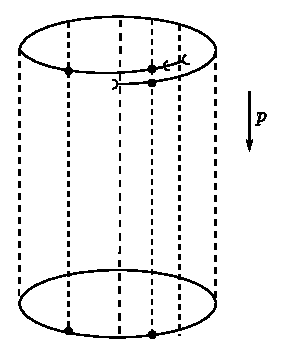
\includegraphics{figures/chap7-fig9.eps}
\end{figure}
\end{remarks*}

\subsection{}\label{chap7:7.5.3}

\begin{prop*}
Let $(M,g)$ be a complete r.m, and let $m$ be a point of $M$ such that
$\exp_{m}$ is of maximal rank everywhere. Then the map $\exp_{m}$ is a
covering map.
\end{prop*}

\begin{proof}
First let us note that $\exp_{m}$ is onto by (\ref{chap7:7.4.8}). By
(\ref{chap3:3.2.1}) $\widehat{g}=(\exp_{m})^{\ast}g$ is a r.s.\@ on the
manifold $T_{m}(M)$. Hence if we prove that $(T_{m}(M),g)$ is complete
then by (\ref{chap7:7.5.1}) we shall be through. Let \pageoriginale $x\in
T_{m}(M)$, $x\neq 0$ and $v:\mathbb{R}\to T_{m}(M)$ be defined by
$v(t)=t.x$. Then $\exp_{m}\circ v$ is a geodesic in $(M,g)$ (because
$(M,g)$ is complete). Hence by (\ref{chap4:4.2.7}), $v$ is a geodesic in
$(T_{m}(M),\widehat{g})$. This being so $\forall \times \in T_{m}(M)$
we have fulfilled condition (iv) of (\ref{chap7:7.4.3}) for $0_{m}\in
T_{m}(M)$. 
\end{proof}

\subsection{}\label{chap7:7.5.4}

\begin{remark*}
If we suppose, in addition to the maximality of rank for $\exp_{m}$
and completeness of $(M,g)$, that $M$ is simply connected then the
above result gives that $\exp_{m}$ is actually a diffeomorphism.
\end{remark*}

\subsection{}\label{chap7:7.5.5}

\begin{coro*}
If $(M,g)$ is complete and simply connected and further\break $A(M)\subset
  ]-\infty$, $0]$ then $M$ is diffeomorphic to $\mathbb{R}^{d}$.
\end{coro*}

\begin{proof}
By (\ref{chap6:6.2.9}) it follows that $\exp_{m}$ is of maximal rank
everywhere for every $m$. Now we have only to apply the above remark.
\end{proof}


\subsection{}\label{chap7:7.5.6}

\begin{remark*}
\begin{itemize}
\item[1)] The completeness assumption on $(M,g)$ cannot be removed as
  the example $((\mathbb{R}^{3}-\{0\}),\can)$ shows.

\item[2)] There is a converse to the above corollary see (\ref{chap8:8.7.2}).
\end{itemize}
\end{remark*}

\section{Closed geodesics}\label{chap7:sec6}

In this article we prove that if $(M,g)$ is a compact r.m, then in
every non-zero free homotopy class there exists a closed geodesic (see
(\ref{chap4:sec5})) the length of which is the least among the lengths of all
paths in that class. Given a non-zero homotopy class, $(M,g)$ being
compact we construct a curve in that class which is of the smallest
length and then show that it is a closed geodesic. Before proceeding
further we recall a few definitions and results. 

\subsection{}\label{chap7:7.6.1}\pageoriginale

\begin{enumerate}
\renewcommand{\labelenumi}{\theenumi)}
\item For any points $m_{1}$ and $m_{2}$ of $M$ let us {\em denote}
  the class of all continuous maps $\sigma$ of $I=[0,1]$ into $M$ such
  that
$$
\sigma(0)=m_{1},\sigma(1)=m_{2}
$$
by $L_{m_{1},m_{2}}$. If $m_{1}$, $m_{2}$ and $m_{3}$ are points of
$M$ and, $\sigma$ and $\zeta$ are elements of $L_{m_{1},m_{2}}$ and
$L_{m_{2},m_{3}}$ respectively then there is an element $\zeta\circ
\sigma\in L_{m_{1},m_{3}}$ which corresponds to the pair
$(\sigma,\zeta)$ in a natural way:
$$
(\zeta\circ\sigma)(t)=
\begin{cases}
\sigma(2t) \text{ if } \circ\leq t\leq \frac{1}{2}\\
\zeta(2t-1)\text{ if } \frac{1}{2}\leq t\leq 1
\end{cases}
$$
If $m_{1}$ and $m_{2}$ are points of $M$ then there is a homotopy
relation in the class $L_{m_{1},m_{2}}:\sigma$ and $\zeta$ in
$L_{m_{1},m_{2}}$ are {\em homotopic} if there exists a map
$$
f:I\times I\to M
$$
such that
$$
f(t,0)=\sigma(t),f(t,1)=\zeta(t) \; \forall t\in I
$$
and $f(0,\alpha)=m_{1}$, $f(1,\alpha)=m_{2} \; \forall \alpha\in I$. {\em
  We denote this by} $\sigma\sim \zeta$.
\end{enumerate}

The particular case when $m_{1}$ and $m_{2}$ coincide is of special
importance for us. In this case, we set $L_{m_{1}}=L_{m_{1},m_{1}}$
and call elements of $L_{m_{1}}$ {\em loops} based at $m_{1}$; in
$L_{m}$ there is a law of composition $\circ$ and the relation
$\sim$. This relation is an equivalence relation in $L_{m}$ and the
law of composition passes down to the quotient set which is denoted by
$\pi_{1}(M,m)$. Further this law of composition in the quotient set
defines the structure of a group on this quotient \pageoriginale
set. $\pi_{1}(M,m)$ is called the {\em fundamental group} of $M$ at
$m$. 

\subsection{}\label{chap7:7.6.2}

\begin{defi*}
Let $m_{1}$, $m_{2}\in M$, $\sigma\in L_{m_{1}}$, $\zeta\in
L_{m_{2}}$. Then they are {\em free homotopic} if there exists a map
$$
f:I\times I\to M
$$
such that
$$
f(t,0)=\sigma(t),f(t,1)=\zeta(t),f(0,\alpha)=f(1,\alpha) \; \forall t\in
I, \forall \alpha \in I.
$$
If this is so then the map $F$:
$$
I\times I\ni (t,\alpha)\to F(t,\alpha)=
\begin{cases}
f(0,3\alpha\cdot t)\text{ if } \; 0\leq t\leq \frac{1}{3}\\
f(3t-1,\alpha)\text{ if } \; \frac{1}{3}\leq t\leq \frac{2}{3}\\
f(0,3(1-t)\cdot\alpha)\text{ if } \; \frac{2}{3}\leq t\leq 1
\end{cases}
$$
is a homotopy between $\sigma$ and $f(0,\alpha)^{-1}\circ\zeta\circ
f(0,\alpha)$, where $f(0,\alpha)\in L_{m_{1},m_{2}}$. {\em The
  quotient set is denoted by} $\oob{F}(M)$; it does not carry a
natural group structure. But it has a zero element, the class of loops
reduced to a point. Conversely if $\gamma$ is a path from $m_{1}$ to
$m_{2}$ and $\Gamma$ is a homotopy between $\sigma$ and
$\gamma^{-1}\circ \zeta\circ\gamma$ then the map $\Phi$:
$$
I\times I\ni (t,\alpha)\to \Phi(t,\alpha)=
\begin{cases}
\gamma(\alpha-3t\cdot\alpha)\text{ if } \;0\leq t\leq \frac{1}{3}\\
\Gamma(3t-1,\alpha)\text{ if }\; \frac{1}{3}\leq t\leq \frac{2}{3}\\
\gamma((3t-2)\cdot\alpha)\text{ if } \;\frac{2}{3}\leq t\leq 1
\end{cases}
$$
is a free homotopy between $\sigma$ and $\zeta$. Hence, we obtain
(\ref{chap7:7.6.3}). An element $\sigma$ of $L_{m_{1}}$ is free homotopic to
an element $\zeta$ of $L_{m_{2}}$ if and only if there exists a path
$\gamma$ from $m_{1}$ to $m_{2}$ such that the loops $\sigma$ and
$\gamma^{-1}\circ \zeta\circ \gamma$ are homotopic. Thus there is a
map
$$
f:\bigcup_{m\in M}\pi_{1}(M,m)\to F(M)
$$
from \pageoriginale $\bigcup\limits_{m\in M}\pi_{1}(M,m)$ into the
free homotopy group of $M$. Further from  
\end{defi*}

\setcounter{subsection}{2}
\subsection{}\label{chap7:7.6.3}
if follows that the image $f(u)$ of an element $u$ in $\pi_{1}(M,m)$
is not zero in $\overline{F}(M)$ if $u$ is not. Further from
(\ref{chap7:7.6.3}) we conclude that for every $a$ in $\overline{F}(M)$, if
we write $a_{m}$ for $\pi_{1}(M,m)\cap f^{-1}(a)$, then 
\begin{equation*}
va_{m}v^{-1}=a_{m} \; \forall v\in \pi_{1}(M,m).\tag{7.6.4}\label{chap7:7.6.4}
\end{equation*}

\setcounter{subsection}{4}
\subsection{}\label{chap7:7.6.5}
3.~Let
$$
p:\widetilde{M}\to M
$$
be the universal covering of $M$. Then let $\sigma$ be an element of
$\pi_{1}(M,m)$, $\widetilde{m}\in p^{-1}(m)$ and $\widetilde{m'}$ be
the end point of the lift $\widehat{\sigma}$ of $\sigma$ through
$\widetilde{m}$. Then $\widetilde{m'}$ depends only on the class of
$\sigma$ in $\pi_{1}(M,m)$, not on $\sigma$ itself. This is related to
the {\em deck transformations} of the covering $p:\widetilde{M}\to M$
as follows: a deck transformation is a map $f:\widetilde{M}\to
\widetilde{M}$ such that $p\circ f=p$; they operate transitively on a
given fibre $p^{-1}(m)$; and there exists a map from $\pi_{1}(M,m)$
into the set of all deck transformations, denoted by $u\to
\widehat{u}$ such that, given $u\in \pi_{1}(M,m)$, then
$\widehat{u}(m)$ is the common end point $\widetilde{m'}$ of lifts
through $\widetilde{m}$ of all loops $\sigma \in u$.

We endow $\widetilde{M}$ with the r.s.\@ $\widetilde{g}=p^{\ast}g$
(see (\ref{chap3:3.2.1}) C) so that $(\widetilde{M},\widetilde{g})\to (M,g)$
is a riemannian covering; and denote by $\widetilde{d}$ the metric
structure of $(\widetilde{M},\widetilde{g})$. Note
$\widetilde{g}=p^{\ast}g$ and $p\circ f=p$ imply
$f^{\ast}\widetilde{g}=\widetilde{g}$, i.e.\@ deck transformations are
isometries.

We fix from now on an $a\in\overline{F}(M)$ such that $a\neq 0$ and
define a function $\varphi$ on $M$ by setting:
$\varphi(m)=\inf\{\widetilde{d}(\widetilde{m},\widehat{u}(\widetilde{m})),
\widetilde{m}\in p^{-1}(m),u\in a\}$ \pageoriginale the geometrical
meaning of which is: $\varphi(m)$ is the infimum of lengths of all
loops in $L_{m}$ whose free homotopy class is in a; we are going to
show that $\varphi$ is continuous on $M$ and that its minimum on the
compact set $M$ is realized by a closed geodesic.

We remark that, for a lift $\widetilde{\sigma}$ in
$(\widetilde{M},\widetilde{g})$ of a curve $\sigma$ in $(M,g)$, we
have: $\lg(\widetilde{\sigma})=\lg(\sigma)$. 

\setcounter{subsection}{5}

\subsection{}\label{chap7:7.6.6}

\begin{lemma*}
Let $m$ be a point of $M$. Then
$$
\varphi(m)=\inf\{\widetilde{d}(\widetilde{m},\widehat{u}(\widetilde{m})|u\in
a_{m}\}\forall \widetilde{m}\in p^{-1}(m).
$$
\end{lemma*}

\begin{proof}
Let $\widetilde{m'}\in p^{-1}(m)$; since deck transformations act
transitively and each deck transformation is induced by an element of
$\pi_{1}(M,m)$, then $\exists\, v\in\pi_{1}(M,m)$ such that
$\widetilde{m'}=\widehat{v}(\widetilde{m})$.

Then we have
$$
\widetilde{d}(\widetilde{m'},\widehat{u}(\widetilde{m'}))=\widetilde{d}(\widehat{v}(\widetilde{m}),\widehat{u}(\widehat{v}(\widetilde{m})))=\widetilde{d}(\widetilde{m},(\widehat{v^{-1}\circ
  u\circ v})(\widetilde{m})) 
$$
since each deck transformation is an isometry. But, by (\ref{chap7:7.6.3}),
$v^{-1}\circ u\circ v\in a_{m}$ for $u\in a_{m}$. Hence the result.
\end{proof}

\subsection{}\label{chap7:7.6.7}

\begin{lemma*}
If $p:(N,h)\to (M,g)$ is an $r$. covering and $(M,g)$ is complete then
$(N,h)$ is complete.
\end{lemma*}

\begin{proof}
We check iii) of (\ref{chap7:7.4.3}); let $y\in U(N)$ and $x=p^{T}(y)$;
the geodesic $t\to{}^{M}\exp(tx)$ is defined for all values of $t$
since $(M,g)$ is complete; its lift in $(N,h)$ is by (\ref{chap4:4.2.7})
nothing but the geodesic $t\to {}^{N}\exp(ty)$, which is therefore
defined for all values of $t$. 
\end{proof}

\subsection{}\label{chap7:7.6.8}

\begin{lemma*}
If $(M,g)$ is complete, then $\forall m\in M$,
$\forall\widetilde{m}\in p^{-1}(m)$, $\exists\, u\in a_{m}$ such that
$\varphi(m)=\widetilde{d}(\widetilde{m},\widehat{h}(\widetilde{m}))$. 
\end{lemma*}

\begin{proof}
By\pageoriginale (\ref{chap7:7.6.6})
$$
\varphi(m)=\inf\{\widetilde{d}(\widetilde{m},\widehat{d}(\widetilde{m}))|u\in
a_{m}\}. 
$$
Looking for an infimum we can work inside a given ball
$\overline{D(m,r)}$ for a suitable $r$, which is compact by
(\ref{chap7:7.5.3}); then $p^{-1}(m)\cap \overline{D(m,r)}$ is a discrete
set in the compact set $\overline{D(m,r)}$, so is finite; a fortiori
the points $\widehat{u}(m)$ in $\overline{D(m,r)}$ are finite in
number. 
\end{proof}

\subsection{}\label{chap7:7.6.9}

\begin{lemma*}
$\varphi$ is continuous on $M$. 
\end{lemma*}

\begin{proof}
Let $m$ be a point of $M$ and let $r$ be a positive real number such
that $B(m,r)$ is a nice ball. Let $n\in B(m,r)$, $\widetilde{m}\in
p^{-1}(m)$. By the proof of (\ref{chap7:7.5.1}) $\exists\,
\widetilde{n}$ with $B(\widetilde{m},r)\cap
p^{-1}(n)=\{\widetilde{n}\}$, and further
$\widetilde{d}(\widetilde{m},\widetilde{n})=d(m,n)$. But $\forall u\in
\pi_{1}(M,m)$: 
$$
\widetilde{d}(\widetilde{m},\widehat{u}(\widetilde{m}))\leq
\widetilde{d}(\widetilde{m},\widetilde{n})+\widetilde{d}(\widetilde{n},\widehat{u}(\widetilde{n}))+\widetilde{d}(\widehat{u}(\widetilde{m}),\widehat{u}(\widetilde{n})) 
$$
and since $\widehat{u}$ is an isometry we have
$$
\widetilde{d}(\widehat{u}(\widetilde{n}),\widehat{u}(\widetilde{m}))=\widetilde{d}(\widetilde{n},\widetilde{m})=d(n,m). 
$$
Hence we have
$$
\widetilde{d}(\widetilde{m},\widehat{u}(\widetilde{m}))\leq
\widetilde{d}(\widetilde{n},\widehat{u}(\widetilde{n}))+2d(m,n)
$$
Hence by the definition of $\varphi$ we have
$$
\varphi(m)\leq\widetilde{d}(\widetilde{n},\widehat{u}(\widetilde{n}))+2d(m,n)
$$
and hence taking the infimum on the right as $u$ varies through
$a_{m}$, 
$$
\varphi(m)\leq \varphi(n)+2d(m,n).
$$
Since $B(m,r)$ is a nice ball we can interchange the roles of $m$ and
$n$ and get
$$
\varphi(n)\leq \varphi(m)+2d(m,n).
$$
Hence
$$
|\varphi(m)-\varphi(n)|\leq 2d(m,n)<2r.
$$
This \pageoriginale holds for any $r$ small enough, so we are through.
\end{proof}

\subsection{}\label{chap7:7.6.10}

\begin{theorem*}
Let $(M,g)$ be a compact r.m., and let $a$ be a non zero free homotopy
class on $M$. Then $\exists\, \gamma\in a$ such that:
\begin{itemize}
\item[\rm i)] $\gamma$ is a closed geodesic,

\item[\rm ii)] $\lg(\xi)\geq \lg(\gamma) \; \forall \zeta\in a$.
\end{itemize}
\end{theorem*}

\begin{proof}
Since $M$ is compact and $\varphi$ is continuous $\exists\, m\in M$
such that
$$
\varphi(m)\leq \varphi(n) \; \forall n\in M.
$$
Let $\widetilde{m}\in p^{-1}(m)$; then by (\ref{chap7:7.6.8}) $\exists\,
u\in a_{m}$ such that
$$
\varphi(m)=\widetilde{d}(\widetilde{m},\widehat{u}(\widetilde{m})).
$$
By (\ref{chap7:7.6.7}) and by (\ref{chap7:7.4.8}),
$\mathscr{T}(\widetilde{m},\widehat{h}(\widetilde{m}))\neq
\emptyset$. Let
$$
\widetilde{\gamma}:[0,1]\to \widetilde{M}, \widetilde{\gamma}\in
\mathscr{T}(\widetilde{m},\widehat{u}(\widetilde{m}));
$$
and set $\gamma=p\circ \widetilde{\gamma}$. We check ii) first: we
have $\lg(\gamma)=\varphi(m)$ by construction. Then let $\tau\in a$
with $\tau\in u$; and let $\widetilde{n}\in p^{-1}(n)$ and
$\widetilde{\tau}$ be the lift of $\tau$ through $\widetilde{n}$. Then
by (\ref{chap7:7.6.6})
$$
\lg(\tau)=\lg(\widetilde{\tau})\geq
\widetilde{d}(\widetilde{n},\widehat{u}(\widetilde{n}))\geq
\varphi(n)\geq \varphi(m)=\lg(\gamma). 
$$
We prove i)~now: we have to prove that $\gamma$ has no
corner. Suppose, by contradiction, that $\gamma$ did have a corner at
$m$; choose a nice ball $B(m,r)$. Suppose, to simplify the notation,
that $m=\gamma(0)=\gamma(1)$; denote by $f_{\epsilon}$ the unique
geodesic in $B(m,r)$ from $\gamma(\epsilon)$ to $\gamma(1-\epsilon)$
(see (\ref{chap7:7.3.1})); because $\gamma'(0)\neq \gamma'(1)$, we have,
by (\ref{chap7:7.3.6}),
$$
\lg(\gamma|[0,\epsilon])+\lg(\gamma|[1-\epsilon,1])<\lg(f_{\epsilon}).
$$
The family of loops $\{f_{\epsilon}\cup
(\gamma|[\epsilon,1-\epsilon])\}$ for $\epsilon\in[0,\epsilon_{0}]$,
with $\epsilon_{0}<r$, is a free homotopy, so $f_{\epsilon_{0}}\cup
(\gamma|[\epsilon_{0},1-\epsilon_{0}])\in a$ and
$\lg(f_{\epsilon_{0}}\cup
(\gamma|[\epsilon_{0},1-\epsilon_{0}])<\lg(\gamma)$,\pageoriginale
contradicting ii),
\begin{figure}[H]
\centering
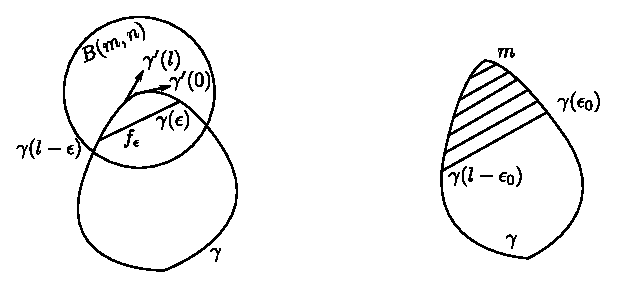
\includegraphics{figures/chap7-fig10.eps}
\end{figure}
\end{proof}

\setcounter{subsection}{10}

\subsection{}\label{chap7:7.6.11}

\begin{remarks*}
\begin{itemize}
\item[1)] Let us note that the compactness condition on $M$ is, in
  general, necessary. For if we take the curve
$$
\{(x,y)\in\mathbb{R}^{2}|y=e^{-x}\}
$$
and take the surface $\sum$ of revolution it generates in
$\mathbb{R}^{3}$ by rotation around the $x$-axis the theorem does not
hold for $\sum$. For the cross sections of the surface by the planes
orthogonal to the $x$-axis are all in the same non zero free-homotopy
class but the infinimum of their lengths $iz$ zero.

\item[2)] From (\ref{chap7:7.6.10}) one sees that if $(M,g)$ is any
  non-simply-connected compact $m$., it has at least one closed
  geodesic. This remains true when this $(M,g)$ is simply connected
  compact but the proof is far more difficult, for it uses Morse
  theory: the oldest proof is in \cite{11} 
\end{itemize}
\end{remarks*}


\section{Manifolds with constant sectional
  curvature}\label{chap7:sec7}\pageoriginale

In (\ref{chap6:sec4}) we have seen that every r.m.\@ of constant sectional
curvature is upto a scalar, locally isometric to one of the three
standard r.m.\@ of constant sectional curvature:
$$
(\mathbb{S}^{d},\can),(\mathbb{R}^{d},\epsilon),(\mathbb{R}^{d},\Hyp).
$$
These standard r.m.s are complete. Use (\ref{chap7:7.4.12}) and the fact
that the geodesics in $(\mathbb{R}^{d},\epsilon)$ are well known (see
\eqref{chap4:4.2.9}). Further they are simply connected. Now we prove that
every simply connected r.m.\@ with constant sectional curvature is
essentially one of the manifolds listed above.

\subsection{}\label{chap7:7.7.1}

\begin{prop*}
Let $(M,g)$ be an r.m.\@ of constant sectional curvature $k$ which is
complete and simply connected. Then $(M,g)$ is isometric to
$$
(\mathbb{R}^{d},(-k)^{-\frac{1}{2}}\cdot
\Hyp)),(\mathbb{R}^{d},\epsilon),
(\mathbb{S}^{d},k^{-\frac{1}{2}}\cdot\can)
$$
$(k<0,k=0,k>0)$.
\end{prop*}

\begin{proof}
Let us denote each of the simply connected r.m.s of constant sectional
curvature by $(N,h)$.
\begin{itemize}
\item[a)] Suppose first that $k\leq 0$. Then by (\ref{chap6:6.2.9})
  $\exp$ has maximal rank everywhere, and hence, by (\ref{chap7:7.5.4}),
  we conclude that for any point $n$ of $N$, $\exp_{n}$ is
  $\infty$-O.K. Let $m$ be any point in $M$. Then, since $(M,g)$ is
  complete, $\exp_{m}$ is defined on the whole of $T_{m}(M)$. Now if
  $u$ is any euclidean isomorphism from $T_{n}(N)$ to $T_{m}(M)$, then
  by the proof of (\ref{chap6:6.4.11}) (see \eqref{chap6:6.4.25}) it follows
  that the map
$$
\lambda=\exp_{m}\circ u\circ \exp^{-1}_{n}
$$
is \pageoriginale a local isometry between $N$ and $M$. Then by
(\ref{chap7:7.5.1}) it follows that $\lambda$ is a covering map. But
since $(M,g)$ is simply connected $\lambda$ is one-one and hence
$\lambda$ is an isomorphism.

\item[b)] Now suppose that $k>0$. Let $n$ be a point of $N$ and let
  $n'\neq n$ and different from the antipodal point of $n$. Then by
  (\ref{chap4:4.5.12}) and (\ref{chap3:3.4.18}) it follows that $\exp_{n}$ and
  $\exp_{n'}$ are $(\pi/\sqrt{k})$-O.K. Now let $m$ be any point of
  $(M,g)$ and let $u:T_{n}(N)\to T_{m}(M)$ be any euclidean
  isomorphism. Then since $(M,g)$ is complete $\exp_{m}$ is defined on
  $T_{m}(M)$ and hence by the proof of Cartan's theorem
  (\ref{chap6:6.4.11}) the map
$$
\lambda={}^{M}\exp_{m}\circ u\circ
({}^{N}\exp_{n}|B(n,\pi/\sqrt{k}))^{-1}
$$
is a local isometry; in particular $\lambda^{T}_{n'}$ is an euclidean
isomorphism, so again
$$
\lambda'={}^{M}\exp_{\lambda(n')}\circ\lambda^{T}_{n'}\circ
({}^{N}\exp_{n'}|B(n',\pi/\sqrt{k}))^{-1} 
$$
is a local isometry.
\end{itemize}
\end{proof}

We claim that $\lambda$, $\lambda'$ coincide on their common domain of
definition, i.e.\@ $B(n,\pi/\sqrt{k})\cap B(n',\pi/\sqrt{k})$. For we
have $\lambda^{T}_{n'}=(\lambda')^{T}_{n'}$ hence the assertion
follows from the diagram (\ref{chap4:4.2.6}).

Now since $B(n,\pi/\sqrt{k})$ together with $B(n',\pi/\sqrt{k})$
covers $N$ and $\lambda$ and $\lambda'$ coincide on the intersection
$B(n,\pi/\sqrt{k})\cap B(n',\pi/\sqrt{k})$ we have a map $\lambda''$
from $N$ to $M$. Since $\lambda$ and $\lambda'$ are local isometries
it follows that $\lambda''$ is. Now if we can show that
$\lambda''(N)=M$ then by (\ref{chap7:7.5.1}) it follows that $\lambda''$
is a covering map, \pageoriginale but since $M$ is simply connected we
get that $\lambda''$ is an isometry. Since $N$ is compact
$\lambda''(N)$ is compact ($M$ is Hausdorff) and hence $\lambda''(N)$
is closed in $M$. But since $\lambda$ and $\lambda'$ are local
isometries and hence in particular open maps we have
$$
\lambda''(N)=\lambda(B(n,\pi/\sqrt{k}))\cup
\lambda'(B(n',\pi/\sqrt{k}))
$$
is open in $M$. But $M$ is connected and hence:
$$
\lambda''(N)=M.
$$

